\subsection[Wykrywalnosc (Jakub Wyka)]{Wykrywalność złośliwego urządzenia USB w konfiguracji karty sieciowej}
\label{subsec:wykrywalnoscJW}

W systemie \textit{Windows} podczas konfiguracji urządzenia pojawia się okienko systemowe opisane wcześniej w
 sekcji~\ref{subsec:wykrywalnoscMK}. Poza nim, po udanej konfiguracji urządzenia wykonującego
 jako karta sieciowa, wyświetla się okno informujące o połączeniu z nową siecią, mimo że
 użytkownik systemu nie łączył się z nią świadomie.
  Jest to prawidłowa reakcja systemu, która może spowodować, że użytkownik, posiadający 
  podstawową wiedzę na temat działania komputera, wykryje złośliwe urządzenie. 


  \begin{figure}[H]
    \centering
    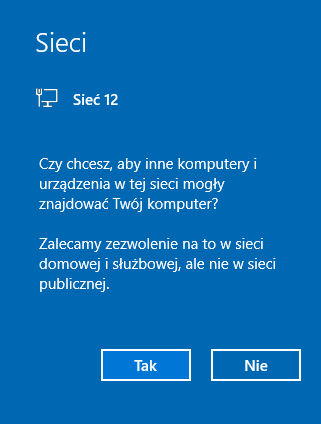
\includegraphics[width=0.5\textwidth]{newcon}
    \caption{Interfejs wyświetlany po udanym połączeniu z nową siecią}
    \label{fig:newcon}
\end{figure}